\documentclass{article}
\usepackage{tikz}
\usepackage{pdfpages}
\usepackage{parskip}
\usepackage{amsmath}
\usepackage[margin=.6in]{geometry}

\begin{document}
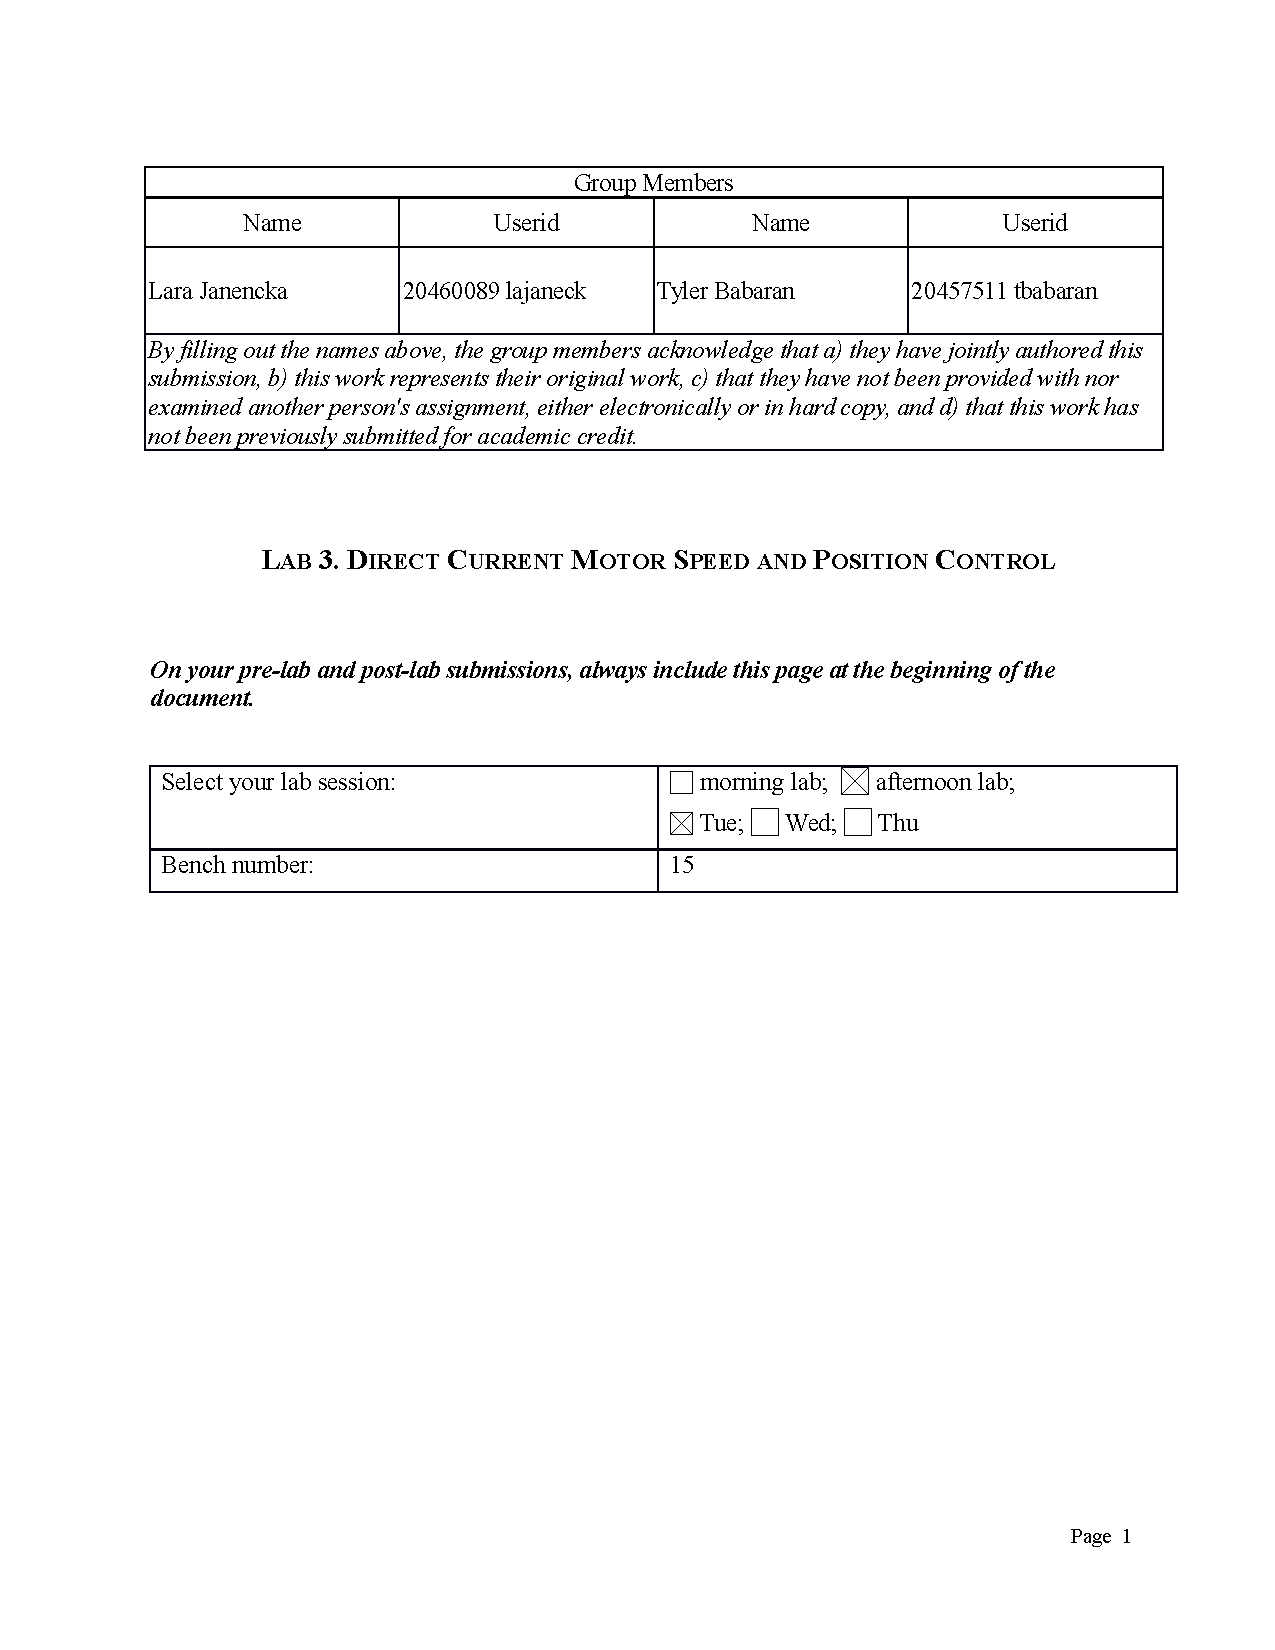
\includepdf[pages={1}]{page1.pdf}
\textbf{Transfer function P(S)}
\begin{align*}
    \text{P(S)}&= \frac{\frac{K_p K_a K}{\tau_m s + 1}}{1 + \frac{K_p K_a K}{\tau_m s + 1}}\\
        &= \frac{K_p K_a K}{\tau_m s + 1 + K_p K_a K}\\
\end{align*}
\textbf{Time constant for P(S)}
\begin{align*}
    \frac{1}{s}\text{P(S)} &= \frac{1}{s} \times \frac{K_p K_a K}{\tau_m s + 1 + K_p K_a K}\\
        &= \frac{1}{s} \times \frac{\frac{K_p K_a K}{1 + K_p K_a K}}{\frac{\tau_m}{1 + K_p K_a K} s + 1}\\
    \tau &= \frac{\tau_m}{1 + K_p K_a K}
\end{align*}
\textbf{Steady-state error for P(S)}
\begin{align*}
    \frac{\text{E(S)}}{\text{V(S)}} &= \frac{1}{1 + \frac{K_p K_a K}{\tau_m s + 1}}\\
        &= \frac{\tau_m s + 1}{\tau_m s + 1 + K_p K_a K}\\
        \text{Since this is stable } & \text{the final value theorem applies}\\
    e_{ss} &= \lim_{t\to\infty} e(t) = \lim_{s\to 0} sE(S)\\
        &= \lim_{s\to 0} s \times \frac{\tau_m s + 1}{\tau_m s + 1 + K_p K_a K} \times \frac{1}{s}\\
        &= \lim_{s\to 0} \frac{\tau_m s + 1}{\tau_m s + 1 + K_p K_a K}\\
        &= \frac{1}{1 + K_p K_a K}\\
\end{align*}
\textbf{Transfer function Q(S)}
\begin{align*}
    \text{Q(S)}&= \frac{\frac{K_p K_a \bar{K}}{s(\tau_m s + 1)}}{1 + \frac{K_p K_a \bar{K}}{s(\tau_m s + 1)}}\\
        &= \frac{K_p K_a \bar{K}}{s(\tau_m s + 1) + K_p K_a \bar{K}}\\
        &= \frac{K_p K_a \bar{K}}{\tau_m s^2 + s + K_p K_a \bar{K}}\\
\end{align*}
\textbf{Steady-state error for Q(S)}
\begin{align*}
    \frac{\text{E(S)}}{\text{V(S)}} &= \frac{1}{1 + \frac{K_p K_a \bar{K}}{s(\tau_m s + 1)}}\\
        &= \frac{s(\tau_m s + 1)}{s(\tau_m s + 1) + K_p K_a \bar{K}}\\
        &= \frac{\tau_m s^2 + s}{\tau_m s^2 + s + K_p K_a \bar{K}}\\
    \text{Since this is stable } & \text{the final value theorem applies}\\
    e_{ss} &= \lim_{t\to\infty} e(t) = \lim_{s\to 0} sE(S)\\
            &=\lim_{s\to 0} \frac{1}{s} \times \frac{\tau_m s^2 + s}{\tau_m s^2 + s + K_p K_a \bar{K}} \times s\\
            &=\lim_{s\to 0} \frac{\tau_m s^2 + s}{\tau_m s^2 + s + K_p K_a \bar{K}}\\
            &= 0
\end{align*}
\textbf{Natural frequency for Q(S)}
\begin{align*}
    Q(S) &= \frac{K_p K_a \bar{K}}{\tau_m s^2 + s + K_p K_a \bar{K}}\\
    \omega_n &= \sqrt{K_p K_a \bar{K}}
\end{align*}
\textbf{Dampening ration for Q(S)}
\begin{align*}
    Q(S) &= \frac{K_p K_a \bar{K}}{\tau_m s^2 + s + K_p K_a \bar{K}}\\
    \zeta &= \frac{1}{2\omega_n}\\
    &= \frac{1}{2\sqrt{K_p K_a \bar{K}}}
\end{align*}
\end{document}
